\chapter{THC-RCCSD method
\label{ch:THC-RCCSD}}

\section{Introduction}
In this chapter we present the first application of our tensor structured 
coupled cluster theory. We start with the RCCSD method, where both two body 
interaction part of the Hamiltonian and ${}^2T$ amplitudes have THC structure. 
This combination of decompositions results in a procedure with quartic cost in 
the basis size $N$ and the ranks of THC approximation.

In THC-RCCSD the decomposition is applied in two different ways. First, a 
THC decomposition of a (constant) two-electron interaction tensor is 
calculated at the beginning of the CC procedure. Second, the factors in the 
THC form of ${}^2T$ are initialized with small random numbers, 
and then updated according to the modified CC iteration we derived in 
Eqn.~\ref{fig:cc_thc_als}. Note that ${}^2T$ is never built as 
a four index tensor, but is rather optimized in a decomposed form.

Diagrammatically, our choice of decompositions in THC-RCCSD can be summarized 
as:
%
\begin{equation}
\vcenter{\hbox{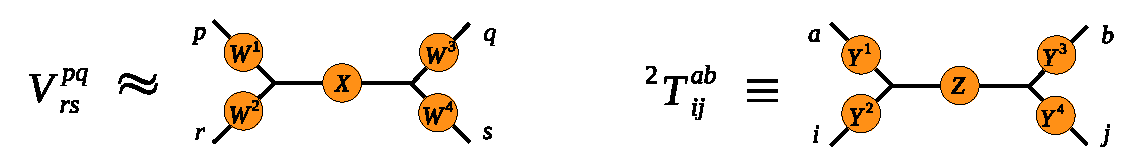
\includegraphics[width=0.9\textwidth]{figures/rccsd_thc_def}}}
.
\label{fig:rccsd_thc_def}
\end{equation}
%
As diagrams show, two electron interaction is decomposed in Mulliken order, as 
well as two body excitation amplitudes. To study the properties of THC-RCCSD 
we calculated energies of a set of small to medium size weakly correlated 
molecules.

\section{Computational details}
In our setup the decomposition of the electron interaction tensor was 
calculated with a two step method, as described in 
Ref.~\cite{schutski2017tensor} First, partial singular value decomposition of 
the integrals in AO basis was calculated. We retained $r_{V}$ singular values 
and vectors. For larger systems, listed in Tab.~\ref{Tab:Energies}, RI 
decomposed two electron integrals were used in place of singular 
vectors. Next, a CP decomposition of rank $r_{V}$ of the resulting 
left and right singular vectors (arranged as three index tensors of size $N 
\times N \times r_{V}$) was calculated with ALS. The iterative least squares 
procedure was stopped when the ratio of the objective function $f$ to the 
square of the Frobenius norm of the original tensor dropped below $10^{-14}$, or 
a limit of 1000 iterations was reached.

In the subsequent coupled cluster calculations we chose the rank of THC 
decomposition of ${}^2T$ amplitudes ($r_{T}$) to be equal to the rank 
used in approximating integrals, e.g. $r_{T} = r_{V}$. 
The CC iterations were stopped either after the energy was converged to within 
$10^{-9}$ Hartree or a limit of 250 iterations 
was reached. All calculations used the cc-pVDZ basis from EMSL
database,\cite{schuchardt2007basis} and the corresponding cc-pVDZ-RI
was used in the RI approximation. The threshold for pseudoinverses was set to 
$10^{-10}$.

Our code was written in MATLAB\cite{matlab} and used Gaussian\cite{gaussian} 
for the calculation of two electron integrals and Hartree Fock solutions. We 
also used Tensorlab\cite{vervliettensorlab} to calculate CPD in the 
decomposition of two electron integrals.

\section{Accuracy of THC for two electron integral approximation}
The accuracy of the THC decomposition of the two-electron integrals governs the
accuracy of the energy in subsequent calculations. Thus, it is important to 
check the dependence of the error in the decomposition of
two-electron integrals on THC rank. Figure~\ref{fig:thc_err_mo_3systems} plots 
this error in a double logarithmic scale for three small molecules. Once again, 
we note that the decomposition is computationally useful if the rank 
$r_\mathrm{V}$ is close to the number of basis functions $N$.  As the figure 
shows, the error in the two-electron integrals decreases exponentially with
respect to THC rank. We found that this trend holds for every system
tested. Further, there is no significant difference whether the two-electron 
integrals are decomposed in the atomic orbital or molecular orbital basis, as 
is demonstrated in Figure~\ref{fig:thc_err_ao_vs_mo}.

%
\begin{figure}[tb]
%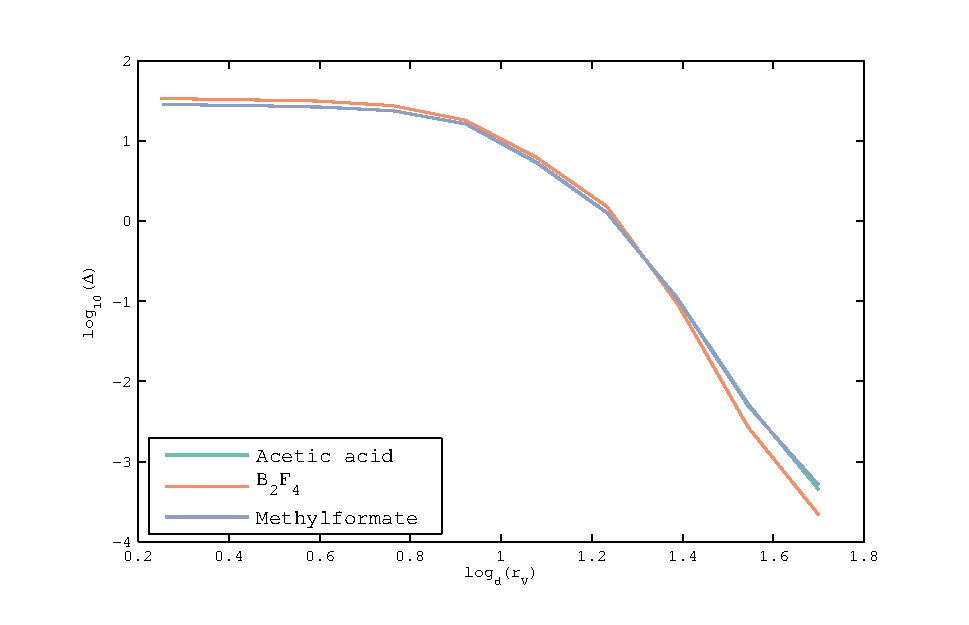
\includegraphics[width=\columnwidth]{figures/thc_err_mo_3systems}
\caption{Frobenius norm of error in decomposed two electron integrals.
\label{fig:thc_err_mo_3systems}}
\end{figure}
%
\begin{figure}[tb]
%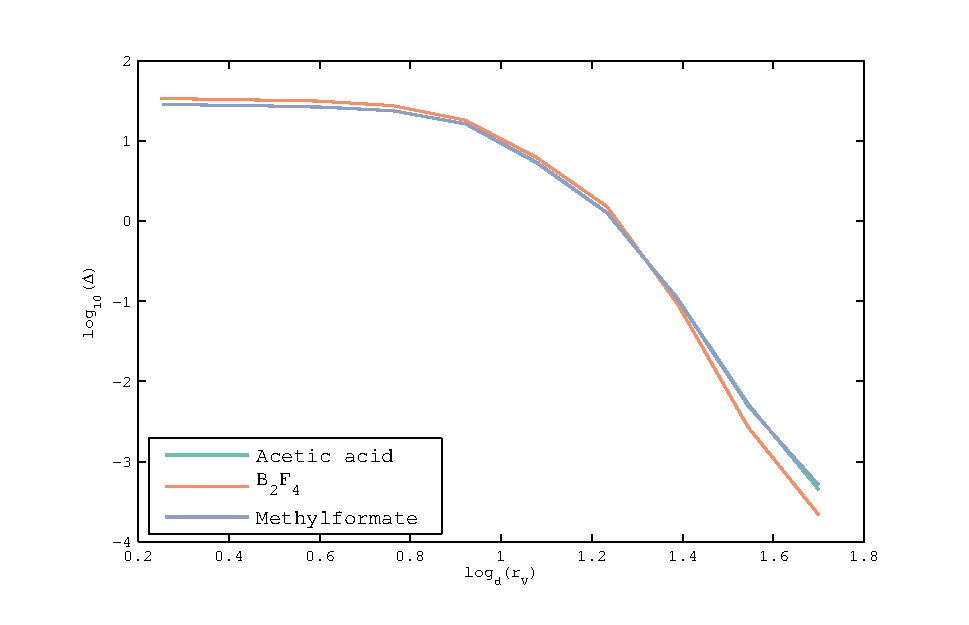
\includegraphics[width=\columnwidth]{figures/thc_err_mo_3systems}
\caption{Frobenius norm of error in decomposed two electron integrals of Acetic 
Acid in atomic and molecular orbital bases.
\label{fig:thc_err_ao_vs_mo}}
\end{figure}
%

To see how these errors of the THC approximation of two-electron 
integrals influence the accuracy of subsequent energies, we checked 
the error in the second-order M{\o}ller-Plesset (MP2) correlation
energy, as shown in Fig.~\ref{fig:mp2_err_ao_full}.  The combination
of MP2 and THC was first proposed by Hohenstein \emph{et
al}.\cite{hohenstein_thc2} and scales as $O(N^4)$.  The way these authors were 
calculating THC decomposition, however, was quite different from ours.
As we found, the error in the MP2 correlation energy follows the trend seen in 
the decomposition of the two-electron integrals (see 
Fig.~\ref{fig:mp2_err_ao_full}). Results within $0.1~mH$
of the exact MP2 correlation energy are already achieved with
$r_\mathrm{V} \sim N^{1.2} - N^{1.4}$.
We expect that the THC would work even better for larger and more extended 
systems as the two-electron integrals become sparser and a lower rank 
decomposition would correspondingly become more accurate.
%
\begin{figure}[tb]
%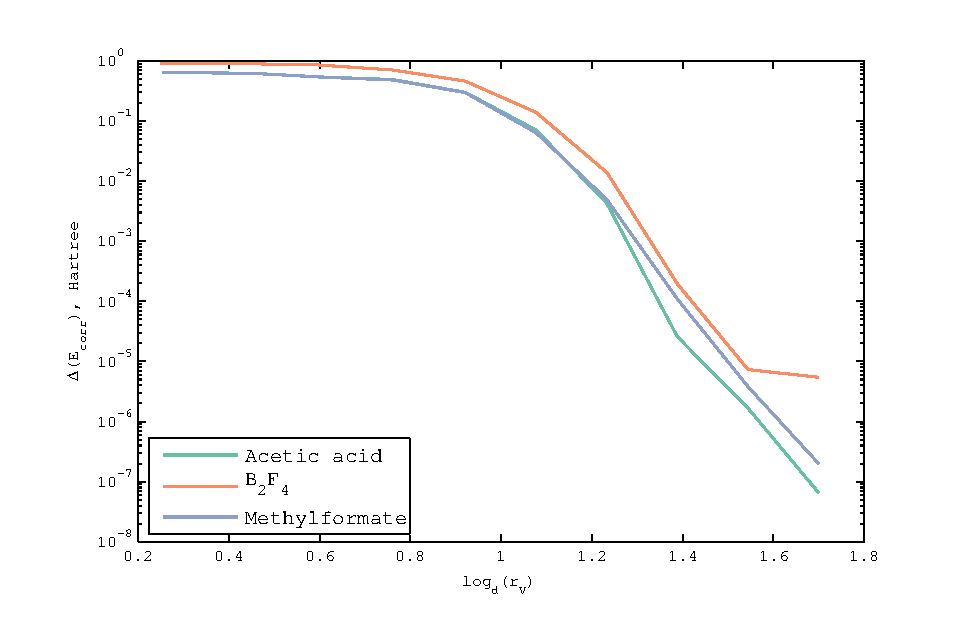
\includegraphics[width=\columnwidth]{figures/mp2_err_ao_full}
\caption{Absolute error in the MP2 correlation energy.
\label{fig:mp2_err_ao_full}}
\end{figure}
%
\section{Accuracy of THC-RCCSD}
We are up to demonstrate the accuracy the THC-decomposed RCCSD
method. Note that we set the rank in THC of amplitudes to equal the rank 
used in the decomposition of two electron integrals. The error in the RCCSD 
correlation energy has a non-monotonic dependence on THC rank, but follows the 
same basic trends as seen in Fig.~\ref{fig:thc_err_mo_3systems} and
Fig.~\ref{fig:mp2_err_ao_full}. Similarly to the case of MP2, errors on 
the order of $0.1~mH$ are achieved with $r_\mathrm{T} = r_\mathrm{V} \sim 
N^{1.2} - N^{1.4}$.
%
\begin{figure}[tb]
%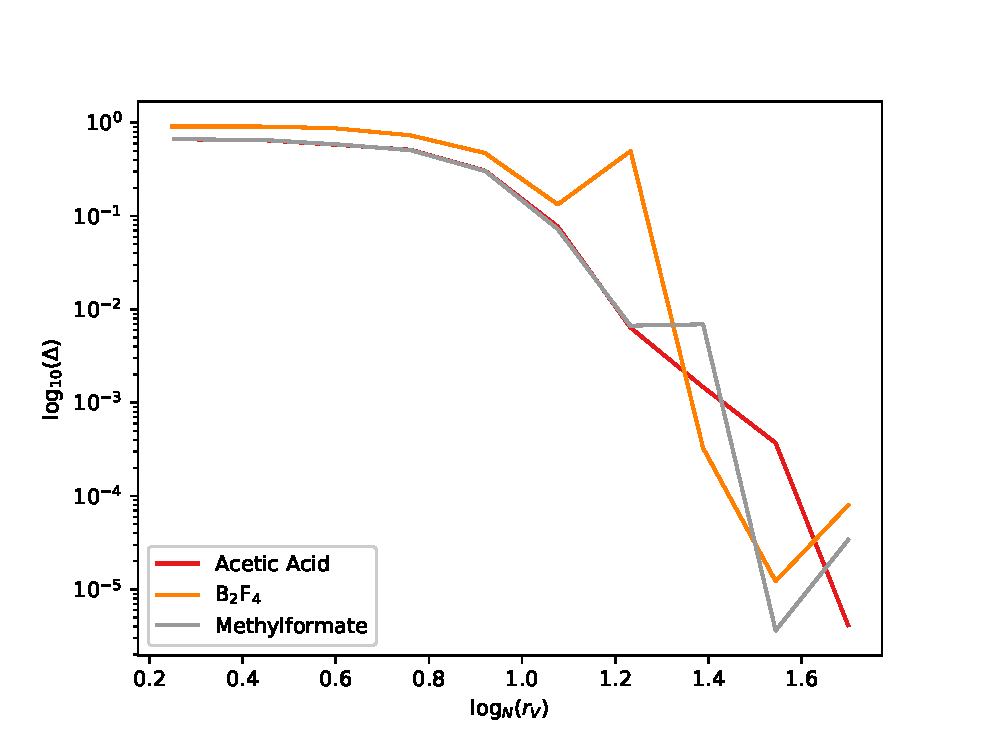
\includegraphics[width=\columnwidth]{figures/cc_err_ao_full}
\caption{Absolute error in the RCCSD correlation energy.
\label{fig:cc_err_ao_full}}
\end{figure}
%
It is interesting to estimate what part of the error in energy can be
attributed to the approximation of the Hamiltonian only. For this reason we 
calculated the correlation energy with converged THC-RCCSD amplitudes but exact
two-electron integrals.  As Fig.~\ref{fig:cc_err_ao_full_amps_only}
shows, using the exact two-electron integrals substantially decreases the error 
in energy, which later motivated us to look for better ways of decomposing the 
two electron integrals. The non-monotonic behavior of the error (as compared to 
MP2) can be attributed to the nonlinear nature of the coupled cluster 
equations, which can be quite sensitive to changes in the parameters of the 
Hamiltonian.
%
\begin{figure}[tb]
%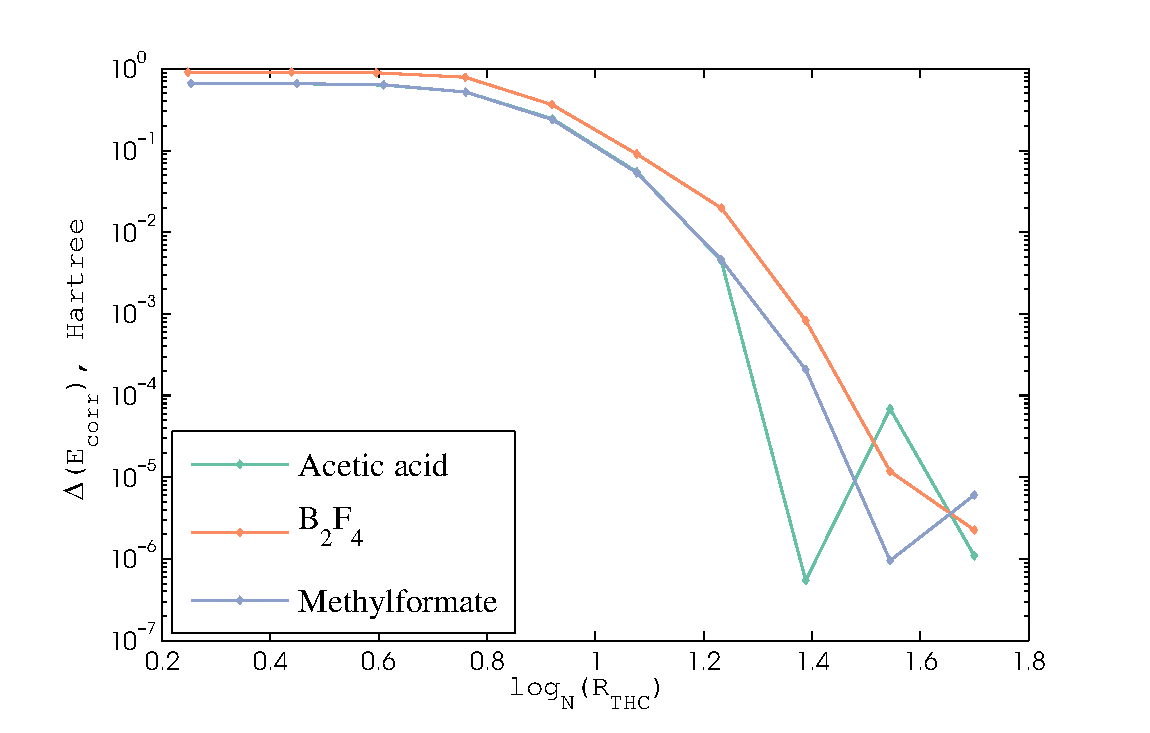
\includegraphics[width=\columnwidth]{figures/cc_err_ao_full_amps_only}
\caption{Absolute error in the RCCSD correlation energy with exact two
electron integrals.
\label{fig:cc_err_ao_full_amps_only}}
\end{figure}
%
\section{{More numerical examples of THC-RCCSD}
\label{sec:more_examples_thc}}
Having checked the properties of THC-RCCSD on few small systems, we 
tested the method on a larger set of small and medium-sized molecules introduced 
in previous work on THC.\cite{hohenstein_thc3} Technical details of the 
calculations, including molecular geometries and reference energies, are 
provided in the supplementary materials of Ref.~\cite{schutski2017tensor}. We 
chose the ranks of the THC decomposition of the amplitudes and integrals to be 
on the same scale as the number of auxiliary basis functions $N_\mathrm{RI}$ 
used in the standard RI approximation. In Table~\ref{Tab:Energies} we list 
energies, differences with respect to regular Coupled Cluster, the number of CC 
iterations and norm of final residuals. We used RI for all these calculations 
in the first step of THC decomposition of the two electron integrals. 
%
\begin{center}
\begin{table}[h]
\caption{CCSD correlation energies ($E_c$), errors in
correlation energies ($\Delta E_c$) 
and the norm of doubles residuals ($|{}^2R_{ij}^{ab}|$) for several small 
molecules.
\label{tab:energies}}
\begin{tabular}{lccccc}
\hline \hline
& & \multicolumn{2}{c}{$\Delta E_c (mH)$} & 
\multicolumn{2}{c}{$|{}^2R_{ij}^{ab}|$}\\
\cline{3-4} \cline{5-6} System & $E_c (mH)$ & $N_\mathrm{RI}$ &
$1.5 \, N_\mathrm{RI}$ & $N_\mathrm{RI}$ &
$1.5 \, N_\mathrm{RI}$\\
\hline
Acetic acid & -666.510 & -0.579 & -0.453 & 0.041 & 0.033 \\
Aniline & -997.193 & -1.177 & -0.471 & 0.051 & 0.032 \\
Diboron tetrafluoride & -909.944 & -0.702 & -0.716 & 0.053 & 0.034\\
Benzene & -823.101 & -0.985 & -0.450 & 0.048 & 0.030\\
Butadiene & -581.340 & -0.710 & -0.274 & 0.041 & 0.025\\
Cyclobutane & -621.099 & -0.895 & -0.290 & 0.039 & 0.028\\
Dimethylsulfoxide & -661.870 & 0.195 & -0.624 & 0.056 & 0.025\\
Furan & -736.463 & -0.865 & -0.454 & 0.046 & 0.033\\
Isobutane & -652.505 & -0.876 & -0.263 & 0.035 & 0.025\\
Methylformate & -666.805 & -0.586 & -0.455 & 0.042 & 0.032\\
Methylnitrite & -708.990 & -0.476 & -0.492 & 0.047 & 0.033\\
Phenol & -1005.727 & -0.887 & -0.514 & 0.051 & 0.032\\
Pyridine & -842.453 & -1.045 & -0.475 & 0.047 & 0.032\\
Pyrrole & -727.051 & -0.855 & -0.407 & 0.045 & 0.032\\
Thiophene & -695.593 & -1.013 & -0.657 & 0.039 & 0.032\\
Toluene & -980.030 & -1.270 & -0.461 & 0.063 & 0.042\\
\hline
MUE\footnote{mean unsigned error} & & 0.820 & 0.466 & &\\
Max\footnote{maximum unsigned error} & & 1.270 & 0.716 & &\\
RMS\footnote{root-mean-square error} & & 0.861 & 0.482 & &\\
\hline\hline
\end{tabular}
\end{table}

\end{center}
%
As the table shows, already with moderate ranks of order of the basis size 
excellent accuracy is attained (differences are below $1 \mathrm{mH}$). The 
error of the approximation decreases as we increase the rank. Let us 
also point to an important finding in Table~\ref{tab:energies}. As THC-RCCSD is 
an approximation to regular CC equations, the full residuals may not be zero, 
because the number of CC equations is usually much larger than the number of 
parameters of THC-RCCSD. An interesting observation is that despite the norm of 
double residuals is not negligible in THC-RCCSD, the error in energy 
is quite low. This contrasts with conventional CC, where the 
difference of energy during iterations with the converged value  
is of the same order as the norm of the residual. This fact is explored in 
more detail in the next chapter. 

\section{Convergence of THC-RCCSD}
Finally, let us discuss the convergence of the THC-RCCSD. In this 
work we used a simple iterative algorithm to solve THC-RCCSD equations, 
and stopped iterations when a specified difference in energy between subsequent 
steps was reached. The convergence of the resulting algorithm significantly 
depends on the rank of the THC approximation. 
Figure~\ref{fig:cc_thc_convergence} shows the number of iterations the 
algorithm had to take to reach $\theta = 1\cdot 10^{6} H$ difference in energy.
%
\begin{figure}[tb]
%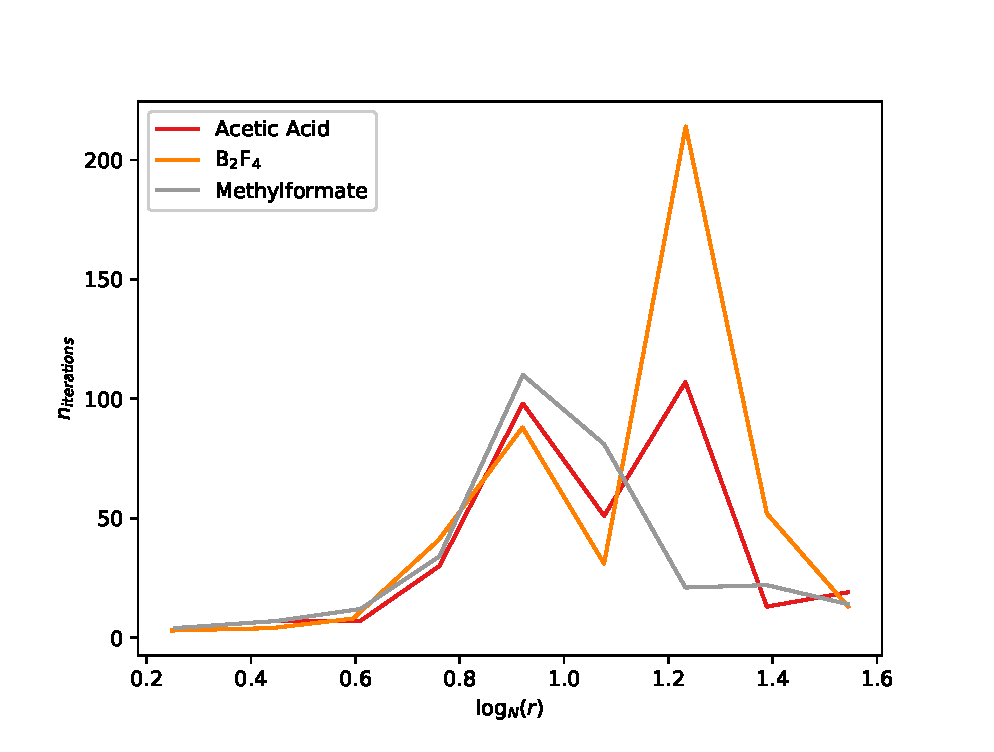
\includegraphics[width=\columnwidth]{figures/niter_vs_logr}
\caption{Number of iterations of THC-RCCSD to reach $1 \cdot 10^{-6} H$ 
difference in energy}
\label{fig:cc_thc_convergence}
\end{figure}
%
For small as well as larger THC ranks the convergence of THC-RCCSD is 
comparable or better than regular RCCSD (if solved by simple iterations). 
In the intermediate regime, however, the algorithm may need
a large number of iterations or fails to converge. We note that the 
convergence in this regime significantly depends on the choice of initial 
parameters. This behavior can possibly be explained by the fact that THC-RCCSD 
in our formulation is a sum of two iterative algorithms, merely, an ALS step and 
a CC iteration. These two parts of THC-RCCSD can generate competing updates, 
depending on the magnitude of the rank. In case of small ranks the update 
should be mostly determined by ALS, as ${}^{2}T$ amplitudes are poorly 
approximated with any set of parameters $Y$. In contrast, with larger ranks 
mostly CC step dominates the update, because ${}^2T$ is well 
approximated at each step. We admit, however, that the means to control 
convergence of our hybrid algorithms may need a further study. All of the 
calculations in Table~\ref{tab:energies} were done in a regime where THC-RCCSD 
performs similarly to regular RCCSD, e. g. where THC ranks are relatively 
large. 

\section{Conclusions}
The development of the THC-RCCSD method is our first application of the tensor 
structured coupled cluster approach.\cite{schutski2017tensor} THC-RCCSD provides 
a viable approximation to conventional RCCSD and should be orders of magnitude 
faster per iteration, especially for large basis sizes $N$. 

It should be noted, however, that most of the time in our 
calculations was spent on the decomposition of the Hamiltonian rather
than on the solution of approximated CC equations. 
One way to overcome this problem is to use quadrature based methods for 
building THC, such as the ones described in Refs.~\cite{hohenstein_thc1} 
and~\cite{parrish2013discrete}. These methods may be much
faster than iterative approaches we employed, at the expense of 
using about 3x larger ranks to reach the same 
accuracy.\cite{parrish2013discrete} Another way is to avoid THC decomposition 
of two electron integrals altogether, as is described in the next 
chapter.

An important aspect not covered in our work on THC-RCCSD is its behavior 
in strong correlation regime. As was mentioned earlier, conventional restricted 
CC methods fail at strong correlation. Our approximate CC methods, however, 
alleviate this problem by providing qualitatively correct solutions, as will be 
shown in Chapter~\ref{ch:CPD-RCCSD}. While not being useful for practical 
calculations, this property of our approximate CC may help to further improve 
future CC algorithms.